
%\newtheorem{definition}[subsection]{Definition}
%\newtheorem{example}[subsection]{Example}
\newtheorem{cor}[subsection]{Corollary}
\newtheorem{pro}[subsection]{Proposition}
\newtheorem{theo}[subsection]{Theorem}
\newtheorem{lem}[subsection]{Lemma}
%\newtheorem{rem}[subsection]{Remark}

\definecolor{main}{HTML}{5989cf}    % setting main color to be used
\definecolor{sub}{HTML}{cde4ff}     % setting sub color to be used

\tcbset{
    sharp corners,
    colback = white,
    before skip = 0.2cm,    % add extra space before the box
    after skip = 0.5cm      % add extra space after the box
}                           % setting global options for tcolorbox

% You can copy any following box you like to your code.
\newtcolorbox{boxA}{
    fontupper = \bf,
    boxrule = 1.5pt,
    colframe = black % frame color
}

\newtcolorbox{boxB}{
    fontupper = \bf\color{main}, % font color
    boxrule = 1.5pt,
    colframe = main,
    rounded corners,
    arc = 5pt   % corners roundness
}
\newtcolorbox{boxC}{
    colback = sub, % background color
    boxrule = 0pt  % no borders
}

\newtcolorbox{boxD}{
    colback = sub, 
    colframe = main, 
    boxrule = 0pt, 
    toprule = 3pt, % top rule weight
    bottomrule = 3pt % bottom rule weight
}

\hypersetup{
    colorlinks=true,
    linkcolor=blue,
    filecolor=magenta,      
    urlcolor=cyan,
    pdftitle={Overleaf Example},
    pdfpagemode=FullScreen,
    }

\urlstyle{same}


\coursetitle{\mtthreeiii}{MT303}
\developers{Wyclife Rao}
\reviewers{Dr Irene Sitawa}
\modulenumber{2}
\modulename{Solutions of Equations of Single Variable}

% courses
\thispagestyle{empty}
\begin{tikzpicture}[overlay,remember picture,font=\sffamily\bfseries]
 \draw[ultra thick,c4,name path=big arc] ([xshift=-2mm]current page.north) arc(150:285:11) coordinate[pos=0.225] (x0);
 \begin{scope}
  \clip ([xshift=-2mm]current page.north) arc(150:285:11) --(current page.north east);
  \fill[c4!50,opacity=0.25] ([xshift=4.55cm]x0) circle (4.55);
  \fill[c4!50,opacity=0.25] ([xshift=3.4cm]x0) circle (3.4);
  \fill[c4!50,opacity=0.25] ([xshift=2.25cm]x0) circle (2.25);
  \draw[ultra thick,c4!50] (x0) arc(-90:30:6.5);
  \draw[ultra thick,c4] (x0) arc(90:-30:8.75);
  \draw[ultra thick,c4!50,name path=arc1] (x0) arc(90:-90:4.675);
  \draw[ultra thick,c4!50] (x0) arc(90:-90:2.875);
  \path[name intersections={of=big arc and arc1,by=x1}];
  \draw[ultra thick,c4,name path=arc2] (x1) arc(135:-20:4.75);
  \draw[ultra thick,c4!50] (x1) arc(135:-20:8.75);
  \path[name intersections={of=big arc and arc2,by={aux,x2}}];
  \draw[ultra thick,c4!50] (x2) arc(180:50:2.25);
 \end{scope} 
 \path[decoration={text along path,text color=c4,
                 raise = -2.8ex,
                 text  along path,
                 text = {},%|\sffamily\bfseries|02/18/2019
                 text align = center,
             },
             decorate
         ] ([xshift=-2mm]current page.north) arc(150:245:11);
 %
 \newcommand\add{4cm}
 \begin{scope}%[shift={(5,0)}]
  \path[clip,postaction={fill=c3}]
  ([xshift=2cm+\add,yshift=-8cm]current page.center) rectangle ++ (4.6,7.7);
  \draw[c5,ultra thick,fill=c2] ([xshift=0.5cm+\add,yshift=-8cm]current page.center)
   ([xshift=0.5cm+\add,yshift=-8cm]current page.center)  arc(180:60:2)
    |- ++ (-3,6) --cycle;
  \draw[ultra thick,c5] ([xshift=-1.5cm+\add,yshift=-8cm]current page.center) 
  arc(180:0:2);
  \draw[ultra thick,c5] ([xshift=0.5cm+\add,yshift=-8cm]current page.center) 
  arc(180:0:2);
  \draw[ultra thick,c5] ([xshift=2.5cm+\add,yshift=-8cm]current page.center) 
  arc(180:0:2);
  \draw[ultra thick,c5] ([xshift=4.5cm+\add,yshift=-8cm]current page.center) 
  arc(180:0:2);
  \fill[white] ([xshift=2.5cm+\add,yshift=-8cm]current page.center) +(60:2) circle(1.5mm)
  node[above
  right=0mm,text=c5!80!black]{$\rho:=\dfrac{1+\sqrt{-3}}{2}$};
 \end{scope}
 %
 \fill[c1] ([xshift=2cm+\add,yshift=-8cm]current page.center) rectangle ++ (-30.7,7.7);
 \node[text=white,anchor=west,scale=2.3,inner sep=0pt] at
 ([xshift=-10cm,yshift=-1.8cm]current page.center) {\color{ulabgold} LEARNING};
 \node[text=white,anchor=west,scale=5,inner sep=0pt] at
 ([xshift=-10cm,yshift=-3.25cm]current page.center) {MODULE \dpmdnumber};
 \node[text=white,anchor=west,scale=2.5,inner sep=0pt,text width=.4\textwidth] at
 ([xshift=-10cm,yshift=-6cm]current page.center) {\dpmdname};
 \node[text=white,anchor=east,scale=2,inner sep=0pt] at
 ([xshift=5.7cm,yshift=-7.5cm]current page.center) {\color{ulabgold}The Open University of Kenya};
 %
% \draw[gray,line width=5mm] 
% ([xshift=2mm,yshift=-1mm]current page.south west) rectangle ([xshift=-2mm,yshift=1mm]current
% page.north east);
\end{tikzpicture}

%\newpage
\pagenumbering{roman}
\thispagestyle{empty}%firstpage


\begin{center}
\vspace*{2cm}
{\Huge\bf BACHELOR OF TECHNOLOGY EDUCATION}\\[3cm]  


%{\fontsize{80}{40}\selectfont \dpcoursecode}\\[2cm]
%
%{\fontsize{30}{40} \selectfont \dpcoursename}\\[2cm]

%\rule{\textwidth}{1pt}
%\vspace{2cm}

%{\fontsize{40}{40}\selectfont \bf Module~\dpmdnumber}\\[2cm]
%
%{\fontsize{30}{40}\selectfont \bf \dpmdname}\\

\vfill
\begin{flushright}
\begin{minipage}{.6\textwidth}
\begin{tcolorbox}%[text ]
\begin{tabular}{ll}%\hline
\subtitle{Developed by:}&\displaydevelopers\\
&\\
\subtitle{Reviewed by:}&\makecell[l]{\displayreviewers}\\
\end{tabular}
\end{tcolorbox}
\end{minipage}\hspace*{-3.5cm}
\end{flushright}
\vspace*{-2.5cm}
\end{center}

\newpage
\thispagestyle{empty}
\null
\vfill
{\renewcommand\arraystretch{1.5}
\begin{tabular}{|l|l|}\hline
\subtitle{Programme Title} & Bachelor of Technology Education \\\hline
\subtitle{Course Title} & \fullcoursename\\\hline
\subtitle{Learning Module number} & Module \dpmdnumber\\\hline
\subtitle{Learning module title} & \dpmdname \\\hline
\subtitle{Module Developer} & \displaydevelopers\\\hline
\subtitle{Reviewed by} & \displayreviewers\\\hline
%\subtitle{Vision} & \vision\\\hline
%\subtitle{Audience description} & \\\hline
\end{tabular}}
\clearpage

%\section{COURSE LEARNING GUIDE}


\subsection*{Preparing for Online and Distance Learning}

This course offers you the opportunity to enter an online space where you can engage with fellow students at the university. The online forums, exercises, tasks and materials have been designed by the course facilitators in such a way that you can draw directly from their knowledge and share in their scholarly interest in online learning and assessment

We hope you will use your access to this virtual classroom to raise all your questions on the course module, to build a network great learners and to share your own thoughts and experiences to the benefit of your fellow students.

   
There are a number of steps you can take to ensure you are well prepared to make the most of this learning opportunity. This resource should prompt you to consider the following:


 \begin{enumerate}[label=\cb$\square$]
   \item How can you best prepare the space where you expect you will spend most of your time engaging in online learning (i.e. in your home or office, or even during your commute to work or whilst traveling)?
  \item   What can you do to ensure you keep working through the course material, even when you do not have Internet access?
    \item How can you familiarise yourself with the course layout, in order to be able to navigate through the steps with ease?
    \item What are the communication strategies and best practices you could consider to best engage with your fellow students and the course facilitators?
    \item What do you do when you need academic or technical support?

 \end{enumerate} 

\subsection*{General Module Guide}

The authors of this module believe that imparting knowledge should always be a mutual relationship between the students and the teachers. Students can actively construct knowledge through experiences gained in reading and answering the learning modules.

You should take time to read everything written in the module, actively and religiously solve all the exercises included to finish this course and be able to gain all the competencies and skills expected to demonstrate the learning outcomes as stated in this course. If you finish with full confidence that you understand and can apply all the knowledge you gain in this course, then you are sure to succeed in tackling the next higher subjects in your chosen course.

In this course, you will be taught not only the knowledge you need to demonstrate your learning outcomes, but you will also gain discipline, perseverance, higher thinking skills, and resourcefulness that would help strengthen your foundation to succeed in life. To successfully finish the course, you must follow the guides set forth in using this module.


\begin{description}[{format=\textcolor{ulabblue}}]
\item[STUDY ENVIRONMENT.]\leavevmode\\
Before engaging into the module, make sure that you are comfortable enough and diminish distractions. Make sure that you develop a study routine to perform and accomplish all the activities set forth by the module.
%\newpage

\item[MODE OF DELIVERY.]\leavevmode\\
Students are required to get a access a digitised copy of the module from the Virtue Learning Environment. As an open and distance learner, you should be able to learn independently and optimise the learning modes and environment available to you as much of  the delivery of all the lessons will be done asynchronously. Your success will greatly depend on your self-motivation and discipline to get your work done without your instructor to remind you from time to time.

\item[STUDY SCHEDULE.] \leavevmode\\
Remember that you have other subjects to attend to, hence, you must manage your time so that you will not be left behind in any of them. Create your own learning plan for each course to make sure that you can perform all the activities. Do not procrastinate your work, remember that time wasted can never be retrieved back. Make sure that even if you are at home, you are a student enrolled in a program, where the learning of all its courses greatly depends on your will to learn as the materials you need are all in your hands. So always be aware of your daily tasks.

\item[PRACTICE EXERCISE.]\leavevmode\\
To measure your learning from your reading, you are given practice exercises which you are supposed to answer daily. This will prepare you in performing your main task.

\item[ONLINE GROUP CHAT.]\leavevmode\\
I am going to create an online Discussion Forum and QA Forum  on the VLE.  This will serve as a room for discussion on the topics and activities found in your module.

\item[RECOMMENDED REFERENCES FOR SUPPLEMENTARY READING.]\leavevmode\\
You are given links that you need to access online. These links are online references such as e-books, online activities, and tutorial videos of the topic. These are other references you can use to further understand the topic and gain additional knowledge and skills.

\item[MAIN TASK.]\leavevmode\\
You are given a task that will require you to apply the knowledge and skills you learned from the module. This can be a group or individual activity which will measure your higher order thinking skills you acquired throughout the topic.

\item[RUBRICS. ]\leavevmode\\
This is a tool to guide you in performing your main task. Through this, you will be able to know the specific indicators that should be found in your task. This is to assess your constructive behaviour towards your learning application. You will be rated according to a 4-point scale shown below.
\begin{center}
{\color{ulabgold} \bf 4 − Excellent\quad\quad   3 −Good\quad\quad    2 − Fair \quad\quad  1 −Poor}
\end{center}
\item[REFLECTIONS.]\leavevmode\\
Writing your reflection will be a passageway to express your experiential learning in using this module. In your honest recall, write everything that you think happened to you during your learning experience in this module. Use the guide questions below:
\begin{description}[{format=\textcolor{ulabblue}}]
\item[First paragraph. ]\leavevmode\\
How was your learning experience? Maybe you can consider describing the effect of the parts of the module (sequence, discussions, examples, practice exercises, online activities, and the main task) in your learning experience. You can point out the strength and weakness of each part so that we can consider it for future improvement of this instructional material.
\item[Second paragraph.  ]\leavevmode\\
What did you learn? Did you successfully acquire the learning outcomes?

\item[Third paragraph.]\leavevmode\\
How can you use what you learned in the future?
\end{description}
\end{description}

\section{ASSESSMENT  TASKS \& EXAMINATION   RULES AND GUIDELINES}

\begin{enumerate}[label=\cb\arabic*.]
\item {\cb SUBMISSION OF ASSESSMENT TASTS.}

Since mathematical skills are best acquired through constant practice, you are encouraged to answer at least two (2) exercises a day. These practice exercises will not be graded but it will help you develop your thinking skills which will prepare you in the performance of your main tasks. You are required to submit your practice exercises every week.
\begin{center} {\cg Usually submission deadlines are set on Saturday 11:59PM EAT} \end{center}

\item  {\cb GROUP CHAT.}

You can post questions, solutions, and comment to other's post. Please be reminded that our group chat is exclusive only for discussion on topics related to this course. Everyone is required to actively participate in the discussions. Also, trolling is highly discouraged. Always observe proper online etiquettes when participating in discussions.
\begin{center} {\cb RULE OF THUMB: ALWAYS THINK BEFORE YOU CLICK} \end{center}

\item  {\cb MAIN TASK. }

Complete documentation during the preparation of your task is required to ensure that every member of the group participated and contributed in the task. May it be photos or screenshots of your virtual meetings or group works. You are going to submit it as attachment of your main task the same way as the practice exercises.



\item {\cb RECOMMENDED REFERENCES FOR SUPPLEMENTARY READING.} 

You can explore online for other references that is related to the topic to gain additional information about the topic. Do not share or post inappropriate materials online or even privately.
\end{enumerate}

\subsection*{Requirements to pass the course}

Compiled Continuous  Assignment/Activities and Tasks  with Final Performance Examination.

\subtitle{Grading System}
\begin{center}
{\renewcommand\arraystretch{1.5}
\begin{tabular}{|l|c|}\hline
Continuous Activities and Tasks  &  50\%\\\hline
Final Performance Examination. &  50\%\\\hline
\end{tabular}
}
\end{center}
%\newpage










%\subsection{INTRODUCTORY MESSAGE}

%A warm welcome to \;  \fullcoursename, {\bf Module on \dpmdname}.



%By this module learning resource, we aim to enable you  achieve the relevant competencies, depict skill, action and purpose successfully. 
 

%It has been designed to provide you with fun and meaningful opportunities for guided and independent learning at your own pace and time. You will be enabled to process the contents of the learning material while being an active learner. Your academic success lies in your own hands.  This module has the following parts and corresponding icons:





{
\renewcommand\arraystretch{4}
\begin{longtblr}{
width=\linewidth,
 colspec={ Q[1,c,f] Q[1.5,r,m] Q[4,l,m] },
%row{1} = { font=\bfseries },
% rowhead = 1,
  caption={ }, 
  label={ },
  rowsep = 4pt,
  hlines = {ulabblue!20, 1pt},
  vlines = {ulabblue!20, 1pt},
}

\includegraphics[width=2cm]{img/audience} & {\bf AUDIENCE}  &  This is a description of a target audience.   \\
{\fontsize{40}{30}\selectfont\color{ulabblue}\faCogs}& {\bf MODULE DESCRIPTION} & 
This part explains the importance of the topics discussed in the module. It will also give you a sneak peek of what you will learn and what is expected from you at the end of the module.\\

\includegraphics[width=2cm]{img/target.png} &  {\bf  EXPECTATION} & These are what you will be able to know after completing the lessons in the module\\

\includegraphics[width=2cm]{img/preactivities} & {\bf PRE-ACTIVITY} &
This activity is to get you set, activate and engage schema to learn the module. Through this activity, you will know the relevance of this activity to the topic that will be discussed in the module.\\

\includegraphics[width=2cm]{img/pretest} &  {\bf PRE - ASSESSMENT} & This will measure your prior knowledge and the concepts to be mastered throughout the lesson. \\

\includegraphics[width=1.7cm]{img/rewind} &  {\bf  RECAP} & This section will measure what learnings and skills that you understand from the previous lesson.\\

\includegraphics[width=1.5cm]{img/lesson} &  {\bf  LESSON} & This section will discuss the topic for this module.\\

\includegraphics[width=2cm]{img/activities} &  {\bf  ACTIVITIES} & This is a set of activities you will perform.\\

\includegraphics[width=2cm]{img/summary} &  {\bf  WRAP UP} & This section summarizes the concepts and applications of the lessons.\\

\includegraphics[width=2cm]{img/discussion}& {\bf DISCUSSIONS} &
This is the meat of the module. The discussion is aligned to the topic learning outcomes that is expected of you to acquire at the end of the module.\\

\includegraphics[width=1.8cm]{img/value} &  {\bf  VALUING} & This part will check the integration of values in the learning competency you will take home.\\

\includegraphics[width=1.8cm]{img/posttest} &  {\bf  POST - ASSESSMENT} & This will measure how much you have learned from the entire module.\\

\includegraphics[width=1.8cm]{img/selfreflect} & {\bf REFLECTION }
&
This part is for you to share your thoughts by writing your reflection, make sure to check your grammar and spelling to ensure the readability and so that it will not alter the thought being delivered. 
\end{longtblr}
}









%\vfill

\audience
\begin{oldactivity}{Audience Description}{
\includegraphics[width=22mm]{img/audience}}{}
This module is offered to all students taking the Bachelor of Technology Education. As an open and distance learner, you should be able to learn independently and optimise the learning modes and environment available to you. Before you begin this course, please confirm the course material, the course requirements and how the course is conducted.
\end{oldactivity}
%\newpage
\pagenumbering{arabic}



\mddescription
This module guides you into a detailed discussion of the concepts of solutions of equations of single variable and interpolation and Lagrange polynomials. Specifically you will learn about
\begin{itemize}
\item error analysis for iterative methods
\item accelerating convergence in iterative methods
\item zeros of polynomials and M\"uller's method
\item interpolation and Lagrange polynomial 
\end{itemize}
%\expectations
%\begin{objenumerate}
%
%\end{objenumerate}

\begin{mlos}
\item Describe key concepts of error types and their impacts on numerical solutions.
\item Summarize methods to accelerate convergence in iterative algorithms.
\item Compute zeros of polynomials using numerical techniques.
\item Evaluate the accuracy of polynomial interpolation using Lagrange polynomials. 
\end{mlos}

\section{Error Analysis for Iterative Methods}
\videolesson
\begin{selfvideo}[1]
%LESSON 3: 
This video presents a discussion on error analysis for iterative processes. Follow the discussion and then solve the problems in the subsequent quiz.
\end{selfvideo}
%\begin{boxB}Question: \end{boxB}
In this section we investigate the order of convergence of functional iteration schemes and, as a means of obtaining rapid convergence, rediscover Newton’s method. We also consider ways of accelerating the convergence of Newton’s method in special circumstances. First, however, we need a new procedure for measuring how rapidly a sequence converges.

\subsection*{ Order of Convergence}
\begin{definition}
Suppose $\displaystyle\left\{p_n\right\}_{n=0}^{\infty}$ is a sequence that converges to $p$, with $p_n\neq p$ for all $n$. If positive constants $\lambda$ and $\alpha$ exist with
\[\lim_{n\rightarrow\infty}\frac{|p_{n+1}-p|}{|p_n-p|^{\alpha}}=\lambda\]
then $\displaystyle\left\{p_n\right\}_{n=0}^{\infty}$ {\bf converges to $p$ of order $\alpha$, with asymptotic error constant $\lambda$.}
\end{definition}

An iterative technique of the form $p_n = g(p_{n-1})$ is said to be of order$\alpha$ if the sequence $\displaystyle\left\{p_n\right\}_{n=0}^{\infty}$ converges to the solution $p = g(p)$ of order $\alpha$.

In general, a sequence with a high order of convergence converges more rapidly than a  sequence with a lower order. The asymptotic constant affects the speed of convergence but not to the extent of the order. Two cases of order are given special attention.
\begin{enumerate}[label=(\roman*)]
\item If $\alpha = 1$ (and $\lambda<1$), the sequence is {\bf linearly convergent}.
\item If $\alpha = 2$, the sequence is {\bf quadratically convergent}.
\end{enumerate}

The next illustration compares a linearly convergent sequence to one that is quadratically convergent. It shows why we try to find methods that produce higher-order convergent sequences.

\begin{example}
Suppose that $\displaystyle\left\{p_n\right\}_{n=0}^{\infty}$  linearly convergent to $0$ with
\[\lim_{n\rightarrow\infty}\frac{|p_{n+1}|}{|p_n|}=0.5\]
 and that $\displaystyle\left\{\tilde{p}_n\right\}_{n=0}^{\infty}$ is quadratically convergent to $0$ with the same asymptotic error constant,
\[\lim_{n\rightarrow\infty}\frac{|\tilde{p}_{n+1}|}{|\tilde{p}_n|^2}=0.5\]
For simplicity we assume that for each $n$ we have
\[\frac{|p_{n+1}|}{|p_n|}\approx0.5\quad\mbox{and}\quad\frac{|\tilde{p}_{n+1}|}{|\tilde{p}_n|^2}\approx0.5.\]
 For the linearly convergent scheme, this means that
\[|p_n-0|=|p_n|\approx0.5|p_{n-1}|\approx(0.5)^2|p_{n-2}|\approx\cdots\approx(0.5)^n|p_0|,\]
whereas the quadratically convergent procedure has
\[\begin{split}
|\tilde{p}_n-0|&=|\tilde{p}_n|\approx0.5|\tilde{p}_{n-1}|^2\approx(0.5)\left[(0.5)|\tilde{p}_{n-2}|^2\right]^2=(0.5)^3|\tilde{p}_{n-2}|^4\\
&\approx(0.5)^3\left[(0.5)|\tilde{p}_{n-3}|^2\right]^4=(0.5)^7|\tilde{p}_{n-3}|^8\\
&\approx\cdots\approx(0.5)^{2^n-1}|\tilde{p}_0|^{2^n}.
\end{split}\]
Table \ref{mod2tab1} illustrates the relative speed of convergence of the sequences to $0$ if $|p_0|=|\tilde{p}_0|=1$.

The quadratically convergent sequence is within $10^{-38}$ of $0$ by the seventh term. At least  $126$ terms are needed to ensure this accuracy for the linearly convergent sequence.\qed
\end{example}

\begin{table}[h]
\centering
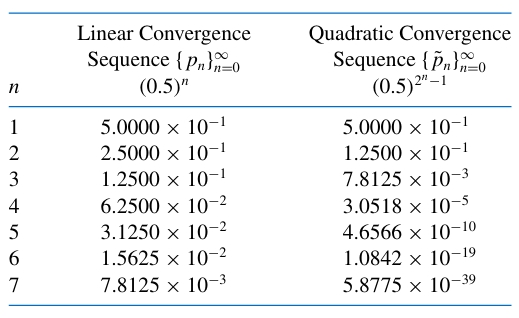
\includegraphics[ width=9cm]{Erroranalysisiterativemethods.jpeg}
\caption{\scriptsize Table 1}
\label{mod2tab1}
\end{table}

Quadratically convergent sequences are expected to converge much quicker than those that converge only linearly, but the next result implies that an arbitrary technique that  generates a convergent sequence does so only linearly.

\begin{theorem}\label{erroranalysisthm1}
Let $g\in C[a,b]$ be such that $g(x)\in[a,b]$, for all $x\in[a,b]$. Suppose, in addition, that $g$ is  continuous on $(a,b)$ and a positive constant $k<1$ exists with
\[|g'(x)|\leq k,\quad\mbox{for all } x\in(a,b).\]
If $g'(p)\neq0$, then for any number $p_0=p$ in $[a,b]$, the sequence
\[p_n=g(p_{n-1}),\quad\mbox{for } n\geq1,\]
converges only linearly to the unique fixed point $p$ in $[a,b]$.
\end{theorem}

Theorem \ref{erroranalysisthm1} implies that higher-order convergence for fixed-point methods of the form $ g(p) = p$ can occur only when $g(p) = 0$. The next result describes additional conditions that ensure the quadratic convergence we seek.

\begin{theorem}\label{erroranalysisthem2}
Let $p$ be a solution of the equation $x = g(x)$. Suppose that $g'(p) = 0$ and $g''$ is continuous with $|g(x)|<M$ on an open interval I containing $p$. Then there exists a $\delta>0$ such that, for $p_0\in[p-\delta, p+\delta]$, the sequence defined by $p_n = g(p_{n-1})$, when $n\geq1$, converges at least quadratically to $p$.  Moreover, for sufficiently large values of $n$,
\[|p_{n+1}-p|<\frac{M}{2}|p_n-p|^2.\]
\end{theorem}
Theorems \ref{erroranalysisthm1} and 2 tell us that our search for quadratically convergent fixed-point methods should point in the direction of functions whose derivatives are zero at the fixed
 point. That is:
\begin{boxB} 
For a fixed point method to converge quadratically we need to have both $g(p) = p$, and $g(p) = 0$.
\end{boxB}

The easiest way to construct a fixed-point problem associated with a root-finding problem $f(x) = 0$ is to add or subtract a multiple of $f(x)$ from $x$. Consider the sequence
\[p_n=g(p_{n-1}),\quad \mbox{for} n\leq1,\]
for $g$ in the form
\[g(x)=x-\phi(x)f(x),\]
 where $\phi$ is a differentiable function that will be chosen later.

For the iterative procedure derived from g to be quadratically convergent, we need to have $g(p) = 0$ when $f(p) = 0$. Because
\[g'(x)=1-\phi'(x)f(x)-f'(x)\phi(x),\]
and $f(p)=0$, we have
\[g'(p)=1-\phi'(p)f(p)-f'(p)\phi(p)=1-\phi'(p)\cdot0-f'(p)\phi(p)=1-f'(p)\phi(p),\]
and $g'(p)=0$ if and only if $\phi(p)=1/f'(p)$.

If we let $\phi(x) = 1/f' (x)$, then we will ensure that $\phi(p) = 1/f'(p)$ and produce the quadratically convergent procedure
\[p_n = g(p_{n-1}) =p_{n-1}-\frac{f(p_{n-1})}{f'(p_{n-1})}.\]
This, of course, is simply Newton’s method. Hence
\begin{boxB} 
If $f(p) = 0$ and $f'(p)= 0$, then for starting values sufficiently close to $p$, Newton’s method will converge at least quadratically.
\end{boxB} 

\subsection*{ Multiple Roots}
In the preceding discussion, the restriction was made that $f'(p)= 0$, where $p$ is the solution to $f(x) = 0$. In particular, Newton’s method and the Secant method will generally give problems if $f'(p) = 0$ when $f(p) = 0$. To examine these difficulties in more detail, we make the following definition.

\begin{definition}
A solution $p$ of $f(x) = 0$ is a {\bf zero of multiplicity} $m$ of $f$ if for $x= p$, we can write $f(x) = (x-p)^mq(x)$, where $lim_{x\rightarrow p}q(x)= 0$.
\end{definition}
In essence, $q(x)$ represents that portion of $f(x)$ that does not contribute to the zero of $f$. The following result gives a means to easily identify {\bf simple} zeros of a function, those that have multiplicity one.

\begin{theorem}\label{erroranalysisthm3}
The function $f\in  C^1[a,b]$ has a simple zero at $p$ in $(a,b)$ if and only if $f(p) = 0$, but $f'(p)= 0$.
\end{theorem}
 The following a generalization of Theorem \ref{erroranalysisthm3}.
\begin{theorem}\label{erroranalysisthm4}

The function $f\in C^m[a,b]$ has a zero of multiplicity $m$ at $p$ in $(a,b)$ if and only if 
\[0=f(p)=f'(p)=f'' (p)=\cdots=f^{(m-1)}(p), \quad\mbox{but}\quad f^{(m)}(p)\neq0.\]
\end{theorem}

The result in Theorem \ref{erroranalysisthm4} implies that an interval about $p$ exists where Newton’s  method converges quadratically to $p$ for any initial approximation $p_0=p$, provided that $p$ is a simple zero. The following example shows that quadratic convergence might not occur if the zero is not simple.

\begin{example}\label{erroranalysisexample1}
Let $f(x)=e^x−x−1$. (a) Show that $f$ has a zero of multiplicity $2$ at $x=0$. (b) Show that  Newton’s method with $p_0=1$ converges to this zero but not quadratically.
\end{example}

\begin{mysolution}
\begin{enumerate}[label=(\alph*)]
\item We have
\[f(x)=e^x−x−1,\qquad f'(x)=e^x−1\qquad \mbox{and}\qquad f''(x)=e^x,\]
so
\[f(0)=e^0−0−1=0,\qquad f'(0)=e^0−1=0 \qquad\mbox{and}\qquad f''(0)=e^0=1.\] 
Theorem \ref{erroranalysisthm4} implies that $f$ has a zero of multiplicity $2$ at $x=0$.
\item The first two terms generated by Newton’s method applied to $f$ with $p_0=1$ are
\[p_1=p_0-\frac{f(p0)}{f'(p_0)} =1-\frac{e-2}{e-1}\approx0.58198,\]
and
\[p_2=p_1-\frac{f(p_1)}{f'(p_1)}\approx0.58198-\frac{0.20760}{0.78957}\approx0.31906.\]
The first sixteen terms of the sequence generated by Newton’s method are shown in Table \ref{table2}. The sequence is clearly converging to $0$, but not quadratically. The graph of $f$ is shown in Figure \ref{pic1}.
\end{enumerate}
\end{mysolution}

\begin{table}[h]
\centering
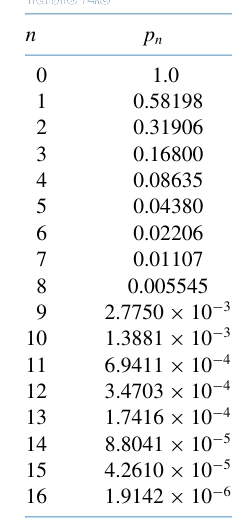
\includegraphics[ width=4cm]{erroranalysistable2.jpeg}
\caption{\scriptsize Table $2$}
\label{table2}
\end{table}

\begin{figure}[h]
\centering
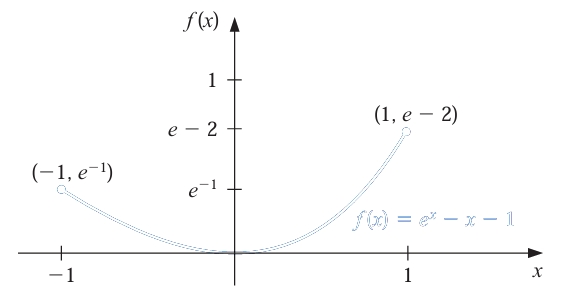
\includegraphics[ width=9cm]{erroranalysispic1.jpeg}
\caption{\scriptsize Figure $1$}
\label{pic1}
\end{figure}

One method of handling the problem of multiple roots of a function $f$ is to define
\[\mu(x)=\frac{f(x)}{f'(x)}.\]
If $p$ is a zero of $f$ of multiplicity $m$ with $f(x)=(x−p)^mq(x)$, then
\[\begin{split}
\mu(x)&=\frac{(x-p)^mq(x)}{m(x-p)^{m-1}q(x)+(x-p)^mq'(x)}\\
 &=(x-p)\frac{q(x)}{mq(x)+(x-p)q'(x)}
\end{split}\]
also has a zero at $p$. However, $q(p)\neq0$, so
\[\frac{q(p)}{mq(p)+(p-p)q'(p)} =\frac1m\neq0,\]
and $p$ is a simple zero of $\mu(x)$. Newton’s method can then be applied to $\mu(x)$ to give
\[g(x)=x-\frac{\mu(x)}{\mu'(x)} =x-\frac{f(x)/f(x)}{\{[f'(x)]^2-[f(x)][f''(x)]\}/[f'(x)]2}\]
which simplifies to
\begin{equation}\label{erroranalysiseqn1}
g(x)=x-\frac{f(x)f'(x)}{[f'(x)]^2-f(x)f''(x)}.
\end{equation}

If $g$ has the required continuity conditions, functional iteration applied to $g$ will be  quadratically convergent regardless of the multiplicity of the zero of $f$. Theoretically, the  only draw back to this method is the additional calculation of $f(x)$ and the more laborious procedure of calculating the iterates. In practice, however, multiple roots can cause serious round-off problems because the denominator of \ref{erroranalysiseqn1} consists of the difference of two numbers that are both close to $0$.


erroranalysisexample1
\begin{example}
In Example \ref{erroranalysisexample1} it was shown that $f(x)=e^x-x-1$ has a zero of multiplicity $2$ at $x=0$ and that Newton’s method with $p_0=1$ converges to this zero but not quadratically. Showt hat the  modification of Newton’s method as given in Equation \ref{erroranalysiseqn1} improves the rate of convergence.
\end{example}

\begin{mysolution}
Modified Newton’s method gives
\[\begin{split}
p_1&=p_0-\frac{f(p_0)f'(p_0)}{f'(p_0)^2-f(p_0)f''(p_0)} \\
&=1-\frac{(e-2)(e-1)}{(e-1)^2-(e-2)e}\approx-2.3421061\times10^{-1}.
\end{split}\]
This is considerably closer to $0$ than the first term using Newton’s method, which was $0.58918$. Table\ref{table3} lists the first five approximations to the double zero at $x=0$. The results were obtained using a system with ten digits of precision. The relative lack of improvement in the last two entries is due to the fact that using this system both the numerator and the denominator approach $0$. Consequently there is a loss of significant digits of accuracy as the approximations approach $0$.
\end{mysolution}

\begin{table}
\centering
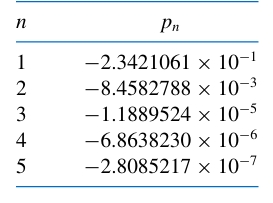
\includegraphics[ width=5cm]{Erroanalysisexampletable3.jpeg}
\caption{\scriptsize Table $3$}
\label{table3}
\end{table}


The following illustrates that the modified Newton’s method converges quadratically  even when in the case of a simple zero.
\begin{example}
In Section $4$ of Module $1$ we found that a zero of $f(x)=x^3+4x^2-10=0$ is $p=1.36523001$. Here we will compare convergence for a simple zero using both Newton’s method and the modified Newton’s method listed in Eq.\ref{erroranalysiseqn1}. Let
\begin{enumerate}[label=(\roman*)]
\item $\displaystyle p_n = p_{n-1}-\frac{p^3_{n-1}+4p^2_{n-1}-10}{3p^2_{n-1}+ 8p_{n-1}}$, from Newton’s method and, from the Modified Newton’s method given by Eq. \ref{erroranalysiseqn1},
\item $\displaystyle p_n = p_{n-1}-\frac{\left(p^3_{n-1}+4p^2_{n-1}-10\right)\left(3p^2_{n-1}+8p_{n-1}\right)}{\left(3p^2_{n-1}+8p_{n-1}\right)^2-\left(p^3_{n-1}+4p^2_{n-1}-10\right)\left(6p_{n-1}+8\right)}$.

With $p_0 = 1.5$, we have
\begin{itemize}
\item[] {\bf Newton's method}
\[ p_1=1.37333333,\quad p_2 = 1.36526201,\quad \mbox{and}\quad p_3 = 1.36523001.\]
\item[] {\bf Modified Newton's method}
\[p_1 = 1.35689898,\quad p_2 = 1.36519585,\quad \mbox{and}\quad p_3 = 1.36523001.\]
\end{itemize}
Both methods are rapidly convergent to the actual zero, which is given by both methods as $p_3$. Note, however, that in the case of a simple zero the original Newton’s method requires substantially less computation.
\end{enumerate}
\end{example}

\begin{myexercise}%\label{Comprehensionquiz2}
Use Newton’s method to find solutions accurate to within $10^{-5}$ to the following problems.
\begin{enumerate}[label=(\alph*)]
\item $x^2 -2xe^{-x} +e^{-2x} = 0$, for $0\leq x \leq1$
\item  $\cos(x + \sqrt{2})+x(x/2+\sqrt{2}) = 0$, for $-2 \leq x \leq-1$
\item $x^3 -3x^2(2^{-x}) + 3x(4^{-x}) - 8^{-x} = 0$, for $0 \leq x \leq 1$
\item $e^{6x} + 3(\ln2)^2e^{2x} - (\ln8)e^{4x} - (\ln2)^3 = 0$, for $-1 \leq x \leq 0$
\end{enumerate}
\begin{mysolution}
\begin{enumerate}[label=(\alph*)]
\item For $p_0=0.5$, we have $p_{13}=0.567135$.
\item For $p_0=-1.5$, we have $p_{23}=-1.414325$.
\item For $p_0=0.5$, we have $p_{22}=0.641166$
\item For$p_0=-0.5$, we have $p_{23}=-0.183274$
\end{enumerate}
\end{mysolution}
\end{myexercise}

\section{Accelerating Convergence}

\begin{youtube}
This video presents a discussion on techniques of accelerating convergence in iterative processes. Follow the discussion and then solve the problems in the subsequent quiz.
\mylink{https://www.youtube.com/watch?v=RYsva1tesvg}
\end{youtube}


\begin{myexercise}%\label{Comprehensionquiz2}
The following sequences are linearly convergent. Generate the first five terms of the sequence $\left\{q_{n}\right\}$ using Aitken's $\Delta^{2}$ method.
\begin{enumerate}[label=(\alph*)]
\item$p_{0}=0.5, \quad p_{n}=\left(2-e^{p_{n-1}}+p_{n-1}^{2}\right) / 3, \quad$ for $n \geq 1$
\item $p_{0}=0.75, \quad p_{n}=\left(e^{p_{n-1}} / 3\right)^{1 / 2}, \quad$ for $n \geq 1$
\item $p_{0}=0.5, \quad p_{n}=3^{-p_{n-1}}, \quad$ for $n \geq 1$
\item $p_{0}=0.5, \quad p_{n}=\cos p_{n-1}, \quad$ for $n \geq 1$ 
\end{enumerate}
\begin{mysolution}
The results are listed in the following table

\begin{center}
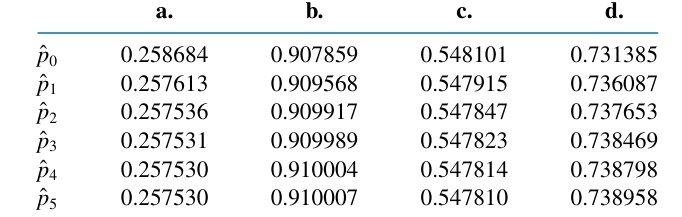
\includegraphics[width=13cm]{Mod2Sec2Comquiz}
\end{center}
\end{mysolution}
\end{myexercise}



\section{Zeroes of Polynomials and M\"uller's Method}
%\activities
%Read on zeros of polynomials and M\"uller's method in pages \textcolor{red}{\bf page $93-100$} of the following reference and then attempt the subsequent quiz
%\begin{activity}[\cg Reading]
%\begin{enumerate}
%\item Burden, R. L., Faires, J. D., Burden, A. M. (2015). Numerical Analysis. Tenth Edition, Cengage Learning.\\
%\end{enumerate}
%\end{activity}

\begin{youtube}
This video presents a discussion on zeros of polynomials and \\M\"uller's method. Follow the discussion and then solve the\\ problems in the subsequent quiz.\\
\mylink{https://www.youtube.com/watch?v=PcGGwhV8PvE\&t=24s}
\end{youtube}



\begin{myexercise}%\label{Comprehensionquiz2}
Find the approximations to within $10^{-4}$ to all the real zeros of the following polynomials using Newton's method.
\begin{enumerate}[label=(\alph*)]
\item $P(x)=x^{3}-2 x^{2}-5$
\item $P(x)=x^{3}+3 x^{2}-1$
\item $P(x)=x^{3}- x-1$
\item $P(x)=x^{4}+2 x^{2}-x-3$
\item $P(x)=x^{3}+4.001 x^{2}+4.002x+1.101$
\item $P(x)=x^{5}-x^{4}+2 x^{3}-3 x^{2}+x-4$
\end{enumerate}
\begin{mysolution}
\begin{enumerate}[label=(\alph*)]
\item For $p_0=1$, we have $p_{22}=2.69065$.
\item For $p_0=1$, we have $p_5=0.53209$; for $p_0=-1$, we have $p_3=-0.65270$; and for $p_0=-3$, we have $p_3=-2.87939$.
\item For $p_0=1$, we have $p_5=1.32472$.
\item For $p_0=1$, we have $p_4=1.12412$; and for $p_0=0$, we have $p_8=-0.87605$.
\item For $p_0=0$, we have $p_6=-0.47006$; for $p_0=-1$, we have $p_4=-0.88533$; and for $p_0=-3$, we have $p_4=-2.64561$.
\item For $p_0=0$, we have $p_{10}=1.49819$.
\end{enumerate}
\end{mysolution}
\end{myexercise}


\section{Interpolation and the Lagrange Polynomial}
\videolesson
\begin{selfvideo}[2]
%LESSON 3: 
This video presents a discussion on interpolation and the Lagrange polynomial. Follow the discussion and then solve the problems in the subsequent quiz.
\end{selfvideo}
%\begin{boxB}Question: \end{boxB}

One of the most useful and well-known classes of functions mapping the set of real numbers into itself is the algebraic polynomials, the set of functions of the form
\[P_{n}(x)=a_{n} x^{n}+a_{n-1} x^{n-1}+\cdots+a_{1} x+a_{0},\]
where $n$ is a nonnegative integer and $a_{0}, \ldots, a_{n}$ are real constants. One reason for their importance is that they uniformly approximate continuous functions. By this we mean that given any function, defined and continuous on a closed and bounded interval, there exists a polynomial that is as ``close'' to the given function as desired. This result is expressed precisely in the Weierstrass Approximation Theorem. (See Figure \ref{Interpolandlagrfig1}.)

\begin{figure}[h]
\centering
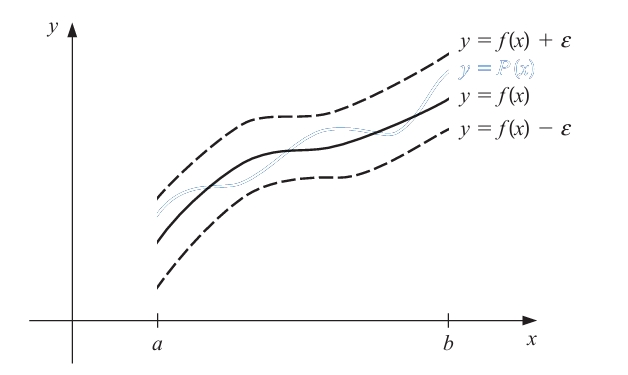
\includegraphics[ width=10cm]{InterpolandLagrfig1.jpeg}
\caption{\scriptsize Figure $2$}
\label{Interpolandlagrfig1}
\end{figure}

\begin{theorem}[Weierstrass Approximation Theorem]
Suppose that $f$ is defined and continuous on $[a, b]$. For each $\epsilon>0$, there exists a polynomial $P(x)$, with the property that
\[|f(x)-P(x)|<\epsilon, \quad \text { for all } x \text { in }[a, b].\]
\end{theorem}
One important reason for considering the class of polynomials in the approximation of functions is that the derivative and indefinite integral of a polynomial are easy to determine and are also polynomials. For these reasons, polynomials are often used for approximating continuous functions.

A class of polynomials that can be considered is the Taylor polynomials which agree as closely as possible with a given function at a specific point, but they concentrate their accuracy near that point. A good interpolation polynomial needs to provide a relatively accurate approximation over an entire interval, and Taylor polynomials do not generally do this. 
%For example, suppose we calculate the first six Taylor polynomials about $x_{0}=0$ for $f(x)=e^{x}$. Since the derivatives of $f(x)$ are all $e^{x}$, which evaluated at $x_{0}=0$ gives 1 , the Taylor polynomials are
%
%Very little of Weierstrass's work was published during his lifetime, but his lectures, particularly on the theory of functions, had significant influence on an entire generation of students.
%
%$$
%\begin{aligned}
%& P_{0}(x)=1, \quad P_{1}(x)=1+x, \quad P_{2}(x)=1+x+\frac{x^{2}}{2}, \quad P_{3}(x)=1+x+\frac{x^{2}}{2}+\frac{x^{3}}{6}, \\
%& P_{4}(x)=1+x+\frac{x^{2}}{2}+\frac{x^{3}}{6}+\frac{x^{4}}{24}, \quad \text { and } \quad P_{5}(x)=1+x+\frac{x^{2}}{2}+\frac{x^{3}}{6}+\frac{x^{4}}{24}+\frac{x^{5}}{120} .
%\end{aligned}
%$$
%
%The graphs of the polynomials are shown in Figure 3.2. (Notice that even for the higher-degree polynomials, the error becomes progressively worse as we move away from zero.)
%
%Figure 3.2\\
%\includegraphics[max width=\textwidth, center]{2025_05_15_4109a88b43049bd640d1g-03}
%
%Although better approximations are obtained for $f(x)=e^{x}$ if higher-degree Taylor polynomials are used, this is not true for all functions. Consider, as an extreme example, using Taylor polynomials of various degrees for $f(x)=1 / x$ expanded about $x_{0}=1$ to approximate $f(3)=1 / 3$. Since
%
%$$
%f(x)=x^{-1}, f^{\prime}(x)=-x^{-2}, f^{\prime \prime}(x)=(-1)^{2} 2 \cdot x^{-3}
%$$
%
%and, in general,
%
%$$
%f^{(k)}(x)=(-1)^{k} k!x^{-k-1}
%$$
%
%the Taylor polynomials are
%
%$$
%P_{n}(x)=\sum_{k=0}^{n} \frac{f^{(k)}(1)}{k!}(x-1)^{k}=\sum_{k=0}^{n}(-1)^{k}(x-1)^{k}
%$$
%
%To approximate $f(3)=1 / 3$ by $P_{n}(3)$ for increasing values of $n$, we obtain the values in Table 3.1-rather a dramatic failure! When we approximate $f(3)=1 / 3$ by $P_{n}(3)$ for larger values of $n$, the approximations become increasingly inaccurate.
%
%Table 3.1
%
%\begin{center}
%\begin{tabular}{c|c|c|c|c|c|c|c|c}
%$n$ & 0 & 1 & 2 & 3 & 4 & 5 & 6 & 7 \\
%\hline
%$P_{n}(3)$ & 1 & -1 & 3 & -5 & 11 & -21 & 43 & -85 \\
%\hline
%\end{tabular}
%\end{center}
%
%For the Taylor polynomials all the information used in the approximation is concentrated at the single number $x_{0}$, so these polynomials will generally give inaccurate approximations as we move away from $x_{0}$. This limits Taylor polynomial approximation to the situation in which approximations are needed only at numbers close to $x_{0}$. For ordinary computational purposes it is more efficient to use methods that include information at various points. We consider this in the remainder of the chapter. 
The primary use of Taylor polynomials in numerical analysis is not for approximation purposes, but for the derivation of numerical techniques and error estimation.

\subsection*{Lagrange Interpolating Polynomials}
The problem of determining a polynomial of degree one that passes through the distinct points $\left(x_{0}, y_{0}\right)$ and $\left(x_{1}, y_{1}\right)$ is the same as approximating a function $f$ for which $f\left(x_{0}\right)=y_{0}$ and $f\left(x_{1}\right)=y_{1}$ by means of a first-degree polynomial {\bf interpolating}, or agreeing with, the values of $f$ at the given points. Using this polynomial for approximation within the interval given by the endpoints is called polynomial {\bf interpolation}.

Define the functions
\[L_{0}(x)=\frac{x-x_{1}}{x_{0}-x_{1}} \quad \text { and } \quad L_{1}(x)=\frac{x-x_{0}}{x_{1}-x_{0}}\]
The linear {\bf Lagrange interpolating polynomial through} ( $x_{0}, y_{0}$ ) and ( $x_{1}, y_{1}$ ) is
\[P(x)=L_{0}(x) f\left(x_{0}\right)+L_{1}(x) f\left(x_{1}\right)=\frac{x-x_{1}}{x_{0}-x_{1}} f\left(x_{0}\right)+\frac{x-x_{0}}{x_{1}-x_{0}} f\left(x_{1}\right).\]
Note that
\[L_{0}\left(x_{0}\right)=1, \quad L_{0}\left(x_{1}\right)=0, \quad L_{1}\left(x_{0}\right)=0, \quad \text { and } \quad L_{1}\left(x_{1}\right)=1,\]
which implies that
\[P\left(x_{0}\right)=1 \cdot f\left(x_{0}\right)+0 \cdot f\left(x_{1}\right)=f\left(x_{0}\right)=y_{0}\]
and
\[P\left(x_{1}\right)=0 \cdot f\left(x_{0}\right)+1 \cdot f\left(x_{1}\right)=f\left(x_{1}\right)=y_{1}\]
So $P$ is the unique polynomial of degree at most one that passes through ( $x_{0}, y_{0}$ ) and $\left(x_{1}, y_{1}\right)$.

\begin{example}
Determine the linear Lagrange interpolating polynomial that passes through the points $(2,4)$ and $(5,1)$.
\end{example}

\begin{mysolution} 
In this case we have
\[L_{0}(x)=\frac{x-5}{2-5}=-\frac{1}{3}(x-5) \quad \text { and } \quad L_{1}(x)=\frac{x-2}{5-2}=\frac{1}{3}(x-2)\]
so
\[P(x)=-\frac{1}{3}(x-5) \cdot 4+\frac{1}{3}(x-2) \cdot 1=-\frac{4}{3} x+\frac{20}{3}+\frac{1}{3} x-\frac{2}{3}=-x+6\]
The graph of $y=P(x)$ is shown in Figure \ref{Lagrangepolynoexample1}.
\end{mysolution}

\begin{figure}[h]
\centering
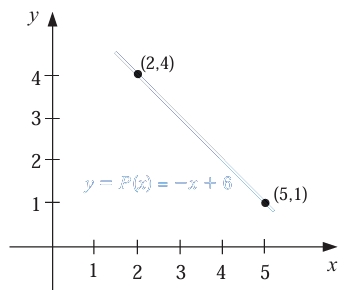
\includegraphics[ width=7cm]{Lagrangepolyexample1.jpeg}
\caption{\scriptsize Figure $3$}
\label{Lagrangepolynoexample1}
\end{figure}

To generalize the concept of linear interpolation, consider the construction of a polynomial of degree at most $n$ that passes through the $n+1$ points
\[\left(x_{0}, f\left(x_{0}\right)\right),\left(x_{1}, f\left(x_{1}\right)\right), \ldots,\left(x_{n}, f\left(x_{n}\right)\right).\]
(See Figure \ref{Lagrangepolynoexplainfig1}.)

\begin{figure}[h]
\centering
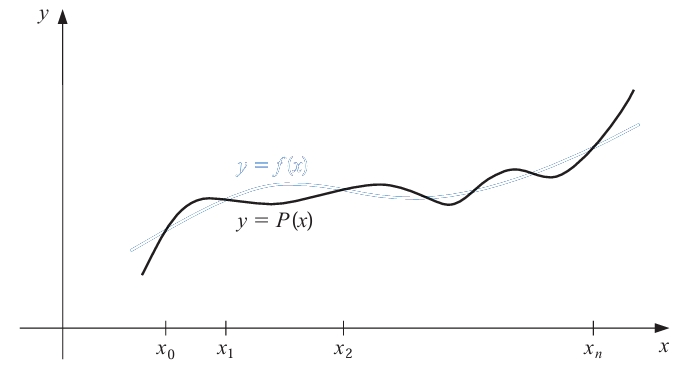
\includegraphics[ width=12cm]{Lagrangepolyexplainfig1.jpeg}
\caption{\scriptsize Figure $4$}
\label{Lagrangepolynoexplainfig1}
\end{figure}

In this case we first construct, for each $k=0,1, \ldots, n$, a function $L_{n, k}(x)$ with the property that $L_{n, k}\left(x_{i}\right)=0$ when $i \neq k$ and $L_{n, k}\left(x_{k}\right)=1$. To satisfy $L_{n, k}\left(x_{i}\right)=0$ for each $i \neq k$ requires that the numerator of $L_{n, k}(x)$ contain the term
\[\left(x-x_{0}\right)\left(x-x_{1}\right) \cdots\left(x-x_{k-1}\right)\left(x-x_{k+1}\right) \cdots\left(x-x_{n}\right).\]
To satisfy $L_{n, k}\left(x_{k}\right)=1$, the denominator of $L_{n, k}(x)$ must be this same term but evaluated at $x=x_{k}$.
Thus
\[L_{n, k}(x)=\frac{\left(x-x_{0}\right) \cdots\left(x-x_{k-1}\right)\left(x-x_{k+1}\right) \cdots\left(x-x_{n}\right)}{\left(x_{k}-x_{0}\right) \cdots\left(x_{k}-x_{k-1}\right)\left(x_{k}-x_{k+1}\right) \cdots\left(x_{k}-x_{n}\right)}.\]
A sketch of the graph of a typical $L_{n, k}$ (when $n$ is even) is shown in Figure \ref{Lagrangepolynoexplainfig2}.

\begin{figure}
\centering
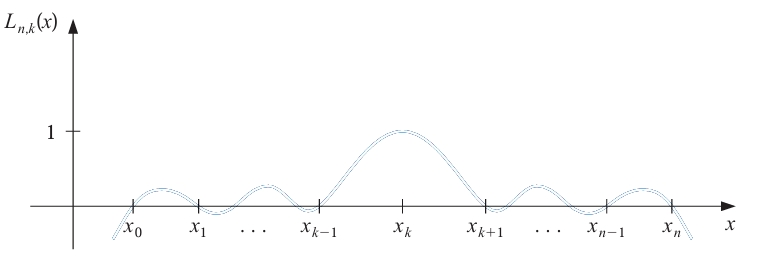
\includegraphics[ width=14cm]{Lagrangepolyexplainfig2.jpeg}
\caption{\scriptsize Figure $5$}
\label{Lagrangepolynoexplainfig2}
\end{figure}

The interpolating polynomial is easily described once the form of $L_{n, k}$ is known. This polynomial, called the $\boldsymbol{n}$ th Lagrange interpolating polynomial, is defined in the following theorem.

\begin{theorem}\label{langrainterpolthm1}
%The interpolation formula named for Joseph Louis Lagrange (1736-1813) was likely known by Isaac Newton around 1675, but it appears to first have been published in 1779 by Edward Waring (1736-1798). Lagrange wrote extensively on the subject of interpolation and his work had significant influence on later mathematicians. He published this result in 1795.
%
%The symbol $\prod$ is used to write products compactly and parallels the symbol $\sum$, which is used for writing sums.
%
If $x_{0}, x_{1}, \ldots, x_{n}$ are $n+1$ distinct numbers and $f$ is a function whose values are given at these numbers, then a unique polynomial $P(x)$ of degree at most $n$ exists with
\[f\left(x_{k}\right)=P\left(x_{k}\right), \quad \text { for each } k=0,1, \ldots, n.\]
This polynomial is given by
\begin{equation}\label{Lagrangepolyexplaineq1}
P(x)=f\left(x_{0}\right) L_{n, 0}(x)+\cdots+f\left(x_{n}\right) L_{n, n}(x)=\sum_{k=0}^{n} f\left(x_{k}\right) L_{n, k}(x), \end{equation}
where, for each $k=0,1, \ldots, n$,
\begin{equation}\label{Lagrangepolyexplaineq2}
\begin{split}
L_{n, k}(x) & =\frac{\left(x-x_{0}\right)\left(x-x_{1}\right) \cdots\left(x-x_{k-1}\right)\left(x-x_{k+1}\right) \cdots\left(x-x_{n}\right)}{\left(x_{k}-x_{0}\right)\left(x_{k}-x_{1}\right) \cdots\left(x_{k}-x_{k-1}\right)\left(x_{k}-x_{k+1}\right) \cdots\left(x_{k}-x_{n}\right)} \\
& =\prod_{\substack{i=0 \\i \neq k}}^{n} \frac{\left(x-x_{i}\right)}{\left(x_{k}-x_{i}\right)}
\end{split}
\end{equation}
\end{theorem}
We will write $L_{n, k}(x)$ simply as $L_{k}(x)$ when there is no confusion as to its degree.

\begin{example}
\begin{enumerate}[label=(\alph*)]
\item Use the numbers (called nodes) $x_{0}=2, x_{1}=2.75$, and $x_{2}=4$ to find the second Lagrange interpolating polynomial for $f(x)=1 / x$.
\item Use this polynomial to approximate $f(3)=1 / 3$.
\end{enumerate}
\end{example}

\begin{mysolution} 
\begin{enumerate}[label=(\alph*)]
\item We first determine the coefficient polynomials $L_{0}(x), L_{1}(x)$, and $L_{2}(x)$. In nested form they are
\[\begin{aligned}
& L_{0}(x)=\frac{(x-2.75)(x-4)}{(2-2.5)(2-4)}=\frac{2}{3}(x-2.75)(x-4) \\
& L_{1}(x)=\frac{(x-2)(x-4)}{(2.75-2)(2.75-4)}=-\frac{16}{15}(x-2)(x-4)
\end{aligned}\]
and
\[L_{2}(x)=\frac{(x-2)(x-2.75)}{(4-2)(4-2.5)}=\frac{2}{5}(x-2)(x-2.75)\]
Also, $f\left(x_{0}\right)=f(2)=1 / 2, f\left(x_{1}\right)=f(2.75)=4 / 11$, and $f\left(x_{2}\right)=f(4)=1 / 4$, so
\[\begin{aligned}
P(x) & =\sum_{k=0}^{2} f\left(x_{k}\right) L_{k}(x) \\
& =\frac{1}{3}(x-2.75)(x-4)-\frac{64}{165}(x-2)(x-4)+\frac{1}{10}(x-2)(x-2.75) \\
& =\frac{1}{22} x^{2}-\frac{35}{88} x+\frac{49}{44}
\end{aligned}\]
\item An approximation to $f(3)=1 / 3$ (see Figure \ref{Lagrangepolynoexample2}) is
\[f(3) \approx P(3)=\frac{9}{22}-\frac{105}{88}+\frac{49}{44}=\frac{29}{88} \approx 0.32955 .\]
%Recall that in the opening section of this chapter (see Table 3.1) we found that no Taylor polynomial expanded about $x_{0}=1$ could be used to reasonably approximate $f(x)=1 / x$ at $x=3$.
\end{enumerate}
\end{mysolution}

\begin{figure}[h]
\centering
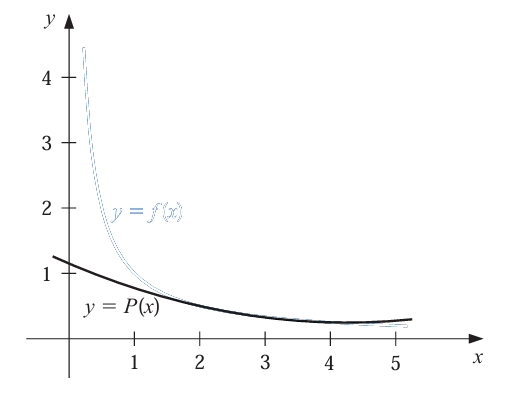
\includegraphics[ width=9cm]{Lagrangepolyexample2.jpeg}
\caption{\scriptsize Figure $6$}
\label{Lagrangepolynoexample2}
\end{figure}

%The interpolating polynomial $P$ of degree less than or equal to 3 is defined in Maple with\\
%$P:=x \rightarrow \operatorname{interp}([2,11 / 4,4],[1 / 2,4 / 11,1 / 4], x)$
%
%$$
%x \rightarrow \operatorname{interp}\left(\left[2, \frac{11}{4}, 4\right],\left[\frac{1}{2}, \frac{4}{11}, \frac{1}{4}\right], x\right)
%$$
%
%To see the polynomial, enter\\
%$P(x)$
%
%$$
%\frac{1}{22} x^{2}-\frac{35}{88} x+\frac{49}{44}
%$$
%
%Evaluating $P(3)$ as an approximation to $f(3)=1 / 3$, is found with evalf( $P(3)$ )
%
%There are other ways that the error term for the Lagrange polynomial can be expressed, but this is the most useful form and the one that most closely agrees with the standard Taylor polynomial error form.
%
%The interpolating polynomial can also be defined in Maple using the CurveFitting package and the call PolynomialInterpolation.
%
The next step is to calculate a remainder term or bound for the error involved in approximating a function by an interpolating polynomial.

\begin{theorem}\label{Lagrangepolyexplaineqthm3}
Suppose $x_{0}, x_{1}, \ldots, x_{n}$ are distinct numbers in the interval $[a, b]$ and $f \in C^{n+1}[a, b]$. Then, for each $x$ in $[a, b]$, a number $\xi(x)$ (generally unknown) between $x_{0}, x_{1}, \ldots, x_{n}$, and hence in ( $a, b$ ), exists with
\begin{equation}
f(x)=P(x)+\frac{f^{(n+1)}(\xi(x))}{(n+1)!}\left(x-x_{0}\right)\left(x-x_{1}\right) \cdots\left(x-x_{n}\right), 
\end{equation}
where $P(x)$ is the interpolating polynomial given in Eq.\ref{Lagrangepolyexplaineq1}.
\end{theorem}
%
%Proof Note first that if $x=x_{k}$, for any $k=0,1, \ldots, n$, then $f\left(x_{k}\right)=P\left(x_{k}\right)$, and choosing $\xi\left(x_{k}\right)$ arbitrarily in ( $a, b$ ) yields Eq. (3.3).
%
%If $x \neq x_{k}$, for all $k=0,1, \ldots, n$, define the function $g$ for $t$ in $[a, b]$ by
%
%$$
%\begin{aligned}
%g(t) & =f(t)-P(t)-[f(x)-P(x)] \frac{\left(t-x_{0}\right)\left(t-x_{1}\right) \cdots\left(t-x_{n}\right)}{\left(x-x_{0}\right)\left(x-x_{1}\right) \cdots\left(x-x_{n}\right)} \\
%& =f(t)-P(t)-[f(x)-P(x)] \prod_{i=0}^{n} \frac{\left(t-x_{i}\right)}{\left(x-x_{i}\right)}
%\end{aligned}
%$$
%
%Since $f \in C^{n+1}[a, b]$, and $P \in C^{\infty}[a, b]$, it follows that $g \in C^{n+1}[a, b]$. For $t=x_{k}$, we have
%
%$$
%g\left(x_{k}\right)=f\left(x_{k}\right)-P\left(x_{k}\right)-[f(x)-P(x)] \prod_{i=0}^{n} \frac{\left(x_{k}-x_{i}\right)}{\left(x-x_{i}\right)}=0-[f(x)-P(x)] \cdot 0=0 .
%$$
%
%Moreover,
%
%$$
%g(x)=f(x)-P(x)-[f(x)-P(x)] \prod_{i=0}^{n} \frac{\left(x-x_{i}\right)}{\left(x-x_{i}\right)}=f(x)-P(x)-[f(x)-P(x)]=0 .
%$$
%
%Thus $g \in C^{n+1}[a, b]$, and $g$ is zero at the $n+2$ distinct numbers $x, x_{0}, x_{1}, \ldots, x_{n}$. By Generalized Rolle's Theorem 1.10, there exists a number $\xi$ in ( $a, b$ ) for which $g^{(n+1)}(\xi)=0$. So
%
%
%\begin{equation*}
%0=g^{(n+1)}(\xi)=f^{(n+1)}(\xi)-P^{(n+1)}(\xi)-[f(x)-P(x)] \frac{d^{n+1}}{d t^{n+1}}\left[\prod_{i=0}^{n} \frac{\left(t-x_{i}\right)}{\left(x-x_{i}\right)}\right]_{t=\xi} \tag{3.4}
%\end{equation*}
%
%
%However $P(x)$ is a polynomial of degree at most $n$, so the $(n+1)$ st derivative, $P^{(n+1)}(x)$, is identically zero. Also, $\prod_{i=0}^{n}\left[\left(t-x_{i}\right) /\left(x-x_{i}\right)\right]$ is a polynomial of degree $(n+1)$, so
%
%$$
%\prod_{i=0}^{n} \frac{\left(t-x_{i}\right)}{\left(x-x_{i}\right)}=\left[\frac{1}{\prod_{i=0}^{n}\left(x-x_{i}\right)}\right] t^{n+1}+(\text { lower-degree terms in } t),
%$$
%
%and
%
%$$
%\frac{d^{n+1}}{d t^{n+1}} \prod_{i=0}^{n} \frac{\left(t-x_{i}\right)}{\left(x-x_{i}\right)}=\frac{(n+1)!}{\prod_{i=0}^{n}\left(x-x_{i}\right)}
%$$
%
%Equation (3.4) now becomes
%
%$$
%0=f^{(n+1)}(\xi)-0-[f(x)-P(x)] \frac{(n+1)!}{\prod_{i=0}^{n}\left(x-x_{i}\right)}
%$$
%
%and, upon solving for $f(x)$, we have
%
%$$
%f(x)=P(x)+\frac{f^{(n+1)}(\xi)}{(n+1)!} \prod_{i=0}^{n}\left(x-x_{i}\right)
%$$

The error formula in Theorem \ref{langrainterpolthm1} is an important theoretical result because Lagrange polynomials are used extensively for deriving numerical differentiation and integration methods. Error bounds for these techniques are obtained from the Lagrange error formula.

Note that the error form for the Lagrange polynomial is quite similar to that for the Taylor polynomial. The $n$th Taylor polynomial about $x_{0}$ concentrates all the known information at $x_{0}$ and has an error term of the form
\[\frac{f^{(n+1)}(\xi(x))}{(n+1)!}\left(x-x_{0}\right)^{n+1}\]
The Lagrange polynomial of degree $n$ uses information at the distinct numbers $x_{0}, x_{1}, \ldots$, $x_{n}$ and, in place of $\left(x-x_{0}\right)^{n}$, its error formula uses a product of the $n+1$ terms $\left(x-x_{0}\right)$, $\left(x-x_{1}\right), \ldots,\left(x-x_{n}\right):$
\[\frac{f^{(n+1)}(\xi(x))}{(n+1)!}\left(x-x_{0}\right)\left(x-x_{1}\right) \cdots\left(x-x_{n}\right)\]

\begin{example}In Example 2 we found the second Lagrange polynomial for $f(x)=1 / x$ on $[2,4]$ using the nodes $x_{0}=2, x_{1}=2.75$, and $x_{2}=4$. Determine the error form for this polynomial, and the maximum error when the polynomial is used to approximate $f(x)$ for $x \varepsilon[2,4]$.
\end{example}

\begin{mysolution}
Because $f(x)=x^{-1}$, we have
\[f^{\prime}(x)=-x^{-2}, \quad f^{\prime \prime}(x)=2 x^{-3}, \quad \text { and } \quad f^{\prime \prime \prime}(x)=-6 x^{-4}.\]
As a consequence, the second Lagrange polynomial has the error form\\
\[\frac{f^{\prime \prime \prime}(\xi(x))}{3!}\left(x-x_{0}\right)\left(x-x_{1}\right)\left(x-x_{2}\right)=-(\xi(x))^{-4}(x-2)(x-2.75)(x-4),\]
for $\xi(x)$ in $(2,4)$. The maximum value of $(\xi(x))^{-4}$ on the interval is $2^{-4}=1 / 16$. We now need to determine the maximum value on this interval of the absolute value of the polynomial
\[g(x)=(x-2)(x-2.75)(x-4)=x^{3}-\frac{35}{4} x^{2}+\frac{49}{2} x-22 .\]
Because
\[D_{x}\left(x^{3}-\frac{35}{4} x^{2}+\frac{49}{2} x-22\right)=3 x^{2}-\frac{35}{2} x+\frac{49}{2}=\frac{1}{2}(3 x-7)(2 x-7),\]
the critical points occur at
\[x=\frac{7}{3}, \text { with } g\left(\frac{7}{3}\right)=\frac{25}{108}, \quad \text { and } \quad x=\frac{7}{2}, \text { with } g\left(\frac{7}{2}\right)=-\frac{9}{16}.\]
Hence, the maximum error is
\[\frac{f^{\prime \prime \prime}(\xi(x))}{3!}\left|\left(x-x_{0}\right)\left(x-x_{1}\right)\left(x-x_{2}\right)\right| \leq \frac{1}{16 \cdot 6}\left|-\frac{9}{16}\right|=\frac{3}{512} \approx 0.00586.\]
\end{mysolution}

The next example illustrates how the error formula can be used to prepare a table of data that will ensure a specified interpolation error within a specified bound.

\begin{example}
Suppose a table is to be prepared for the function $f(x)=e^{x}$, for $x$ in $[0,1]$. Assume the number of decimal places to be given per entry is $d \geq 8$ and that the difference between adjacent $x$-values, the step size, is $h$. What step size $h$ will ensure that linear interpolation gives an absolute error of at most $10^{-6}$ for all $x$ in $[0,1]$ ?
\end{example}

\begin{mysolution}
Let $x_{0}, x_{1}, \ldots$ be the numbers at which $f$ is evaluated, $x$ be in $[0,1]$, and suppose $j$ satisfies $x_{j} \leq x \leq x_{j+1}$. Eq. (3.3) implies that the error in linear interpolation is
\[|f(x)-P(x)|=\left|\frac{f^{(2)}(\xi)}{2!}\left(x-x_{j}\right)\left(x-x_{j+1}\right)\right|=\frac{\left|f^{(2)}(\xi)\right|}{2}\left|\left(x-x_{j}\right)\right|\left|\left(x-x_{j+1}\right)\right|.\]
The step size is $h$, so $x_{j}=j h, x_{j+1}=(j+1) h$, and
\[|f(x)-P(x)| \leq \frac{\left|f^{(2)}(\xi)\right|}{2!}|(x-j h)(x-(j+1) h)|\]
Hence
\[\begin{aligned}
|f(x)-P(x)| & \leq \frac{\max _{\xi \in[0,1]} e^{\xi}}{2} \max _{x_{j} \leq x \leq x_{j+1}}|(x-j h)(x-(j+1) h)| \\
& \leq \frac{e}{2} \max _{x_{j} \leq x \leq x_{j+1}}|(x-j h)(x-(j+1) h)|
\end{aligned}\]

Consider the function $g(x)=(x-j h)(x-(j+1) h)$, for $j h \leq x \leq(j+1) h$. Because
\[g^{\prime}(x)=(x-(j+1) h)+(x-j h)=2\left(x-j h-\frac{h}{2}\right),\]
the only critical point for $g$ is at $x=j h+h / 2$, with $g(j h+h / 2)=(h / 2)^{2}=h^{2} / 4$.

Since $g(j h)=0$ and $g((j+1) h)=0$, the maximum value of $\left|g^{\prime}(x)\right|$ in $[j h,(j+1) h]$ must occur at the critical point which implies that
\[|f(x)-P(x)| \leq \frac{e}{2} \max _{x_{j} \leq x \leq x_{j+1}}|g(x)| \leq \frac{e}{2} \cdot \frac{h^{2}}{4}=\frac{e h^{2}}{8}.\]
Consequently, to ensure that the the error in linear interpolation is bounded by $10^{-6}$, it is sufficient for $h$ to be chosen so that
\[\frac{e h^{2}}{8} \leq 10^{-6}. \text { This implies that } h<1.72 \times 10^{-3}.\]
Because $n=(1-0) / h$ must be an integer, a reasonable choice for the step size is $h=0.001$.
\end{mysolution}
\begin{myexercise}%\label{Comprehensionquiz2}
For the given functions $f(x)$, let $x_{0}=0, x_{1}=0.6$, and $x_{2}=0.9$. Construct interpolation polynomials of degree at most one and at most two to approximate $f(0.45)$, and find the absolute error.
\begin{multicols}{2}
\begin{enumerate}[label=(\alph*)]
\item $f(x)=\cos x$
\item $f(x)=\sqrt{1+x}$
\item $\quad f(x)=\ln (x+1)$
\item $f(x)=\tan x$
\end{enumerate}
\end{multicols}

\begin{mysolution}
\begin{enumerate}[label=(\alph*)]
\item $P_1(x)=-0.148878x+1$; $P_2(x)=-0.452592x^2-0.0131009x+1$; $P_1(0.45)=0.933005$;
 $|f(0.45)-P_1(0.45)|=0.032558$; $P_2(0.45)=0.902455$; $|f(0.45)-P_2(0.45)|=0.002008$
\item $P_1(x)=0.467251x+1$; $P_2(x)=-0.0780026x^2+0.490652x+1$; $P_1(0.45)=1.210263$;
 $|f(0.45)-P_1(0.45)|=0.006104$; $P_2(0.45)=1.204998$; $|f(0.45)-P_2(0.45)|=0.000839$
\item $P_1(x)=0.874548x$; $P_2(x)=-0.268961x^2+0.955236x$; $P_1(0.45)=0.393546$; $|f(0.45)-P_1(0.45)|=0.0212983$; $P_2(0.45)=0.375392$; $|f(0.45)-P_2(0.45)|=0.003828$
\item $P_1(x)=1.031121x$; $P_2(x)=0.615092x^2+0.846593x$; $P_1(0.45)=0.464004$; $|f(0.45)-P1(0.45)|=0.019051$; $P_2(0.45)=0.505523$; $|f(0.45)-P2(0.45)|=0.022468$
\end{enumerate}
\end{mysolution}
\end{myexercise}


%\discussion


\begin{posttest}[\textcolor{red}{End of Module 2 Quiz}]
\item Use the modified Newton’s method given as 
\[g(x)=x-\frac{f(x)f'(x)}{{[f'(x)]^2-[f(x)][f''(x)]}/[f'(x)]^2}\]
to find solutions accurate to within $10^{-5}$ to the following problems. Is there an improve
ment in speed or accuracy over Comprehension Quiz for section $1$?
\begin{enumerate}[label=(\alph*)]
\item $x^2 -2xe^{-x} +e^{-2x} = 0$, for $0\leq x \leq1$
\item  $\cos(x + \sqrt{2})+x(x/2+\sqrt{2}) = 0$, for $-2 \leq x \leq-1$
\item $x^3 -3x^2(2^{-x}) + 3x(4^{-x}) - 8^{-x} = 0$, for $0 \leq x \leq 1$
\item $e^{6x} + 3(\ln2)^2e^{2x} - (\ln8)e^{4x} - (\ln2)^3 = 0$, for $-1 \leq x \leq 0$
\end{enumerate}
\item Let $g(x) = \cos(x -1)$ and $p^{(0)}_0 =2$. Use Steffensen’s method to find $p^{(1)}_0$.
\item Find the approximations to within $10^{-4}$ to all the real zeros of the following polynomials using M\''uler's method.
\begin{enumerate}[label=(\alph*)]
\item $P(x)=x^{3}-2 x^{2}-5$
\item $P(x)=x^{3}+3 x^{2}-1$
\item $P(x)=x^{3}- x-1$
\item $P(x)=x^{4}+2 x^{2}-x-3$
\item $P(x)=x^{3}+4.001 x^{2}+4.002x+1.101$
\item $P(x)=x^{5}-x^{4}+2 x^{3}-3 x^{2}+x-4$
\end{enumerate}
\item Use Theorem \ref{Lagrangepolyexplaineqthm3} to find an error bound for the approximations in the Comprehension Quiz for Section $4$.
\begin{mysolution}
\begin{enumerate}[label=\arabic*.]
\item
\begin{enumerate}[label=(\alph*)]
\item For $p_0=0.5$, we have $p_{3}=0.567143$.
\item For $p_0=-1.5$, we have $p_{2}=-1.414158$
\item For $p_0=0.5$, we have $p_3=0.641274$.
\item For$p_0=-0.5$, we have $p_5=-0.183319$.
\end{enumerate}
These figures show an improvement in speed and accuracy.
\item $p^{(1)}_0 =0.826427$
\item The following table lists the initial approximation and the roots.
\begin{center}
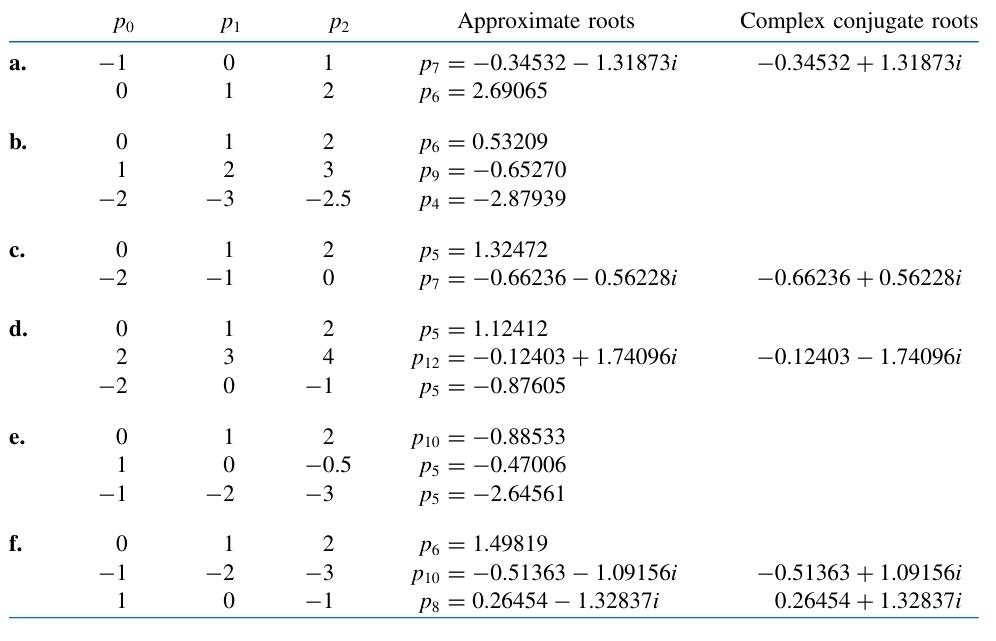
\includegraphics[width=15cm]{EndofMod2Q3sol}
\end{center}
\item 
\begin{enumerate}[label=(\alph*)]
\item $\left|\frac{f''(\xi)}{2} (0.45-0)(0.45-0.6)\right|\leq0.135$; $\left|\frac{f'''(\xi)}{6}(0.45-0)(0.45-0.6)(0.45-0.9)\right|\leq0.00397$\\
\item $\left|\frac{f''(\xi)}{2} (0.45-0)(0.45-0.6)\right|\leq0.03375$; $\left|\frac{f'''(\xi)}{6}(0.45-0)(0.45-0.6)(0.45-0.9)\right|\leq0.001898$\\
\item $\left|\frac{f''(\xi)}{2} (0.45-0)(0.45-0.6)\right|\leq0.135$; $\left|\frac{f'''(\xi)}{6}(0.45-0)(0.45-0.6)(0.45-0.9)\right|\leq0.010125$\\
\item $\left|\frac{f''(\xi)}{2} (0.45-0)(0.45-0.6)\right|\leq0.06779$; $\left|\frac{f'''(\xi)}{6}(0.45-0)(0.45-0.6)(0.45-0.9)\right|\leq0.151$
\end{enumerate}
\end{enumerate}
\end{mysolution}
\end{posttest}

%share your understanding of properties of functions and their applications to solving rates of change problems in physical phenomenon 


%\end{actsoln}

\takehome

\comy{You are now at the last part of this module. Your  task is to do a self-reflection on your learning experience. In ypur own words describe what you have learnt in this module.}



\references
\begin{refenumerate}
\item Kong, Q., Siauw, T., Bayen, A., (2020). Python Programming and Numerical Methods. First Edition, Academic Press,  ISBN-13 ‏ : ‎ 978-0128195499 \\
\mylink{https://pythonnumericalmethods.studentorg.berkeley.edu/notebooks/Index.html}
%chapter 1 pg 7-36 functions\\
%chapter 1 pg 51-83 limits and continuity\\
%chapter 1 pg 45-50 rates of change\\
%chapter 2 pg 108-120 the derivative\\
%\item Mendelson, E. (2022). Schaum's Outline of Calculus. McGraw-Hill Education.
%chapter 6 51-55 functions
%chapter 7 59-65 limits
%chapter 8 69-74 continuity
%chapter 9 77-81 derivative
%\item Calculus \mylink{https://math.libretexts.org/Bookshelves/Calculus}
%\item Chris McMullen, 2021, Essential Calculus Skills Practice Workbook with Full Solutions, Zishka Publishing, ISBN 978-1-941691-24-3
%\item R. Adams and C. Essex, 2021, Calculus: A complete Course, Addison Wesley, ISBN 13: 978-0135732588
%\item P. Abbott and H. Neill, 2018, Calculus: A Complete Introduction: The Easy Way to Learn Calculus (Teach Yourself), ISBN 13: 978-1473678446
\end{refenumerate}





%\wrapup
%To wrap-up, answer the following questions:
%
%\begin{enumerate}
%\item 
%%when do we say that a limit of a function exists?
%%\item how do we remove discontinuity in functions?
%%\item what is the relationship between the gradient of the tangent line and the derivative?
%\end{enumerate}
















%\newpage

%\facilitation


%
\begin{center}
    {\Large \textbf{FUNCTIONS OF SEVERAL VARIABLES}}\\[2mm]
(DEFINITION, DOMAIN, RANGE, GRAPHS AND LEVEL CURVES) \\[4mm]

\mycenterbox{5 minute review}%\\[4mm]
Recap the definition of a function of several variables, and the meaning of domain, range, graph and level curves of functions of several variables.
\end{center}
\mycenterbox{Warm-up.}%\\[4mm]
\problemAnswer{
Match the function with its graph (labeled I–VI).Give reasons for your choices
\begin{multicols}{3}
\begin{enumerate}[label=(\alph*)]
\item $f(x,y)=|x|+|y|$\\[4mm]
\item $f(x,y)=|xy|$
\item $f(x,y)=\frac{1}{1+x^2+y^2}$\\2mm]
\item $f(x,y)=(x^2-y^2)^2$
\item $f(x,y)=(x-y)^2$\\[4mm]
\item $f(x,y)=\sin(|x|+|y|)$
\end{enumerate}
\end{multicols}

\begin{center}
%\centering
\includegraphics[width=10cm]{MCTutorial1Q1.JPEG}
\end{center}
%\tcbox[tcbox raise base]{Warm-up}
 
%\begin{flushright}
%\begin{tikzpicture}
%    % A body
%
%
%    % Non-rectangle shapes must be drawn as polygone
%    \begin{scope}[shift={(3,0)}]
%        \draw  (0,0.5) -- (0,4) -- (.5,4) -- (.5,4.5) -- (1.,4.5) -- (4.,4.5) --(4.,4)-- (4.5,4) --(4.5,0.5) --(4.0,0.5)--(4.0,0.0)-- (.5,0) --(0.5,0.5) -- cycle;
%        % Draw symmetry lines
%        \draw [symmetry] (.5, 0.5) -- (.5,4.0);
%        \draw [symmetry] (4, 0.5) -- (4,4.0);
%        \draw [symmetry] (.5,4.0) -- (4,4.0);
%         \draw [symmetry] (.5, 0.5) -- (4, 0.5);
%        % Dimensions
%        \draw (4.5,0) -- ++(0.5,0) coordinate (D1) -- +(5pt,0);
%        \draw (4.5,4.5) -- ++(0.5,0) coordinate (D2) -- +(5pt,0);
%        \draw [dimen] (D1) -- (D2) node {6cm};
%       
%        
%        \draw (0.0,5) -- ++(0,0.5) coordinate (D1) -- +(0,+5pt);
%        \draw (0.5,5) -- ++(0,0.5) coordinate (D2) -- +(0,+5pt);
%        \draw [dimen,-] (D1) -- (D2) node [above=5pt] {$x$ cm};
%        \draw [dimen,<-] (D1) -- ++(-5pt,0);
%        \draw [dimen,<-] (D2) -- ++(+5pt,0);
%    \end{scope}
%\end{tikzpicture}
%\end{flushright}

}


\mycenterbox{Problems.}%

%\begin{center}
%\tcbox[tcbox raise base]{ Problems. Choose from the below}
%\end{center}
\problem{Exploring functions}%
\begin{enumerate}[(a)]
\item Are the following functions even, odd, or neither? What can you say
about their range?
\begin{multicols}{4}
 \begin{enumerate}[(i)]
\item $\displaystyle \frac{3x}{x^2+2}$
\item $\displaystyle \cos x+3$
\item $\displaystyle \frac{2x^3}{\cos x+3}$
\item $\displaystyle \frac{3x^4+2x^2}{\sin x+4}$
\end{enumerate}
\end{multicols}
\item Consider the functions $\sin^n x$ and $\cos^n x$, where $n$ is a positive integer.
Which are odd, which are even, and what are their periodicities?
\item What is the periodicity of $f(x) = 2 \cos x+\sin 2x$? Is it even/odd/neither?

\end{enumerate}

\problem{Cubic functions} 
Show that $x-1$ is a factor of the cubic function%
$$P(x)=x^3-2x^2-5x+6,$$
and  find the quadratic factor $Q(x)$ such that $P(x) = (x -1)Q(x)$. Factorise
$Q(x)$ and hence sketch $P(x).$

%\newpage
\problem{Sigmoid functions*.}%
For positive integers $n$, consider the family of functions
$$\displaystyle f_n= \frac{x^n}{2^n+x^n}.$$
\begin{enumerate}[(a)]
\item What are appropriate domains and ranges for $f_n(x)$? Do they depend on $n$?

\item Is $f_n(x)$ even, odd, or neither? Does this depend on $n$?

\item Show that for $x\geq 0$, $f_n(x)$ are strictly increasing functions and that
$0\leq f_n(x) < 1.$
\item What is the value of $f_n(2)$? Does it depend on $n$?

\item By considering the values of $f_n(1.9)$ and $f_n(2.1)$ for $n = 2, 4, 8, 16, 32$ and
$64$, show that the graph of $f_n(x)$ for $x\ge 0$ is an increasing sigmoid (that
is, $S$-shaped) function that approaches a step function as $n\rightarrow \infty$.
\end{enumerate}

\mycenterbox{Selected answers and hints}%

For the warm-up, $V(x)=4x(3-x)^2$. Writing $x=1+\epsilon$, we get
$$V = 4(1 +\epsilon)(3- (1+\epsilon))^2=4(4-\epsilon^2(3-\epsilon)).$$
If $-1<\epsilon<2$ then $\epsilon^2 (3-\epsilon)\ge 0$, with equality when $\epsilon=0$. Thus the maximum
value of $V$ occurs when $\epsilon= 0$, i.e. $x = 1\rm{cm}$.

\begin{enumerate}
\item 
\begin{enumerate}[(i)]
\item Odd. The range is the interval  $[-\frac{3}{4}\sqrt{2},\; \frac{3}{4}\sqrt{2}]$
\item Even. The range is the interval $[2, 4]$.
\item Odd. The range is all of $\mathbb R$.
\item Neither. (For example, writing $\displaystyle \frac{5}{\sin x+4}$ we have $\displaystyle f(1)= \frac{5}{\sin (1)+4} \equiv 1.032 (3\rm{dp})$ which is neither $f(1)$ nor $-f(1)$.)\\[4mm]
The range is the nonnegative reals $[0,\infty)$

\end{enumerate}
\end{enumerate}










